%pdflatex black.tex
% black background
%convert -density 150x150 -background black -alpha remove -alpha off black.pdf black.png
\documentclass[border={2pt 2pt 2pt 2pt}]{standalone}
\usepackage{tikz}
\usetikzlibrary{calc}
\begin{document}

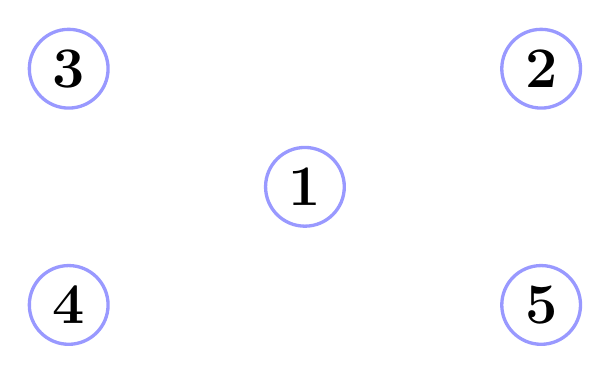
\begin{tikzpicture}
\coordinate (A) at (3,0);
\coordinate (B) at (6,1.5);
\coordinate (C) at (0,1.5);
\coordinate (D) at (0,-1.5);
\coordinate (E) at (6,-1.5);
\draw[white,ultra thick] (A)--(B)--(E)--cycle (A)--(C)--(D)--cycle;
\draw[blue!40,very thick,fill=white] (A) circle [radius=0.5];
\draw[blue!40,very thick,fill=white] (B) circle [radius=0.5];
\draw[blue!40,very thick,fill=white] (C) circle [radius=0.5];
\draw[blue!40,very thick,fill=white] (D) circle [radius=0.5];
\draw[blue!40,very thick,fill=white] (E) circle [radius=0.5];
\node at (A) {\huge\bf 1};
\node at (B) {\huge\bf 2};
\node at (C) {\huge\bf 3};
\node at (D) {\huge\bf 4};
\node at (E) {\huge\bf 5};
\end{tikzpicture}

\end{document}
